\documentclass[10pt,journal,compsoc]{IEEEtran}

\usepackage{cite}
% correct bad hyphenation here
\hyphenation{op-tical net-works semi-conduc-tor}
\usepackage[utf8]{inputenc} %para introdução de caracteres especiais
\usepackage[english]{babel}
\usepackage{tikz}
\usepackage{scalefnt}
\usepackage{comment} 
\usepackage{graphicx}

\begin{document}

\title{Wall Following STDR}
\author{\^{A}ngela Cardoso~and~In\^{e}s Caldas%
\thanks{Faculdade de Engenharia da Universidade do Porto, Rua Dr. Roberto Frias, 4200-465 Porto, Portugal.}}

\IEEEtitleabstractindextext{%
\begin{abstract}
The abstract goes here.
\end{abstract}

% Note that keywords are not normally used for peerreview papers.
\begin{IEEEkeywords}
The keywords go here.
\end{IEEEkeywords}}


% make the title area
\maketitle


%%%%%%%%%%%%%%%%
% INTRODUCTION %
%%%%%%%%%%%%%%%%
\section{Introduction}
The most basic types of robotic systems are purely reactive. These systems do not have neither the ability to form memories, nor to use past experiences to inform current decisions. Since they are fast and rely only on the current sensor readings, instead of an accurate map, the use of which requires very accurate localization capabilities, reactive approaches are often used for robot navigation. However, reactive navigation does not plan ahead and is therefore susceptible to local minima. 

In this project we developed a stable wall follower behavior for a simple reactive robot. The design, implementation and testing of our solution, were made with the support of the \textit{ROS} framework and the \textit{STDR Simulator} package. The robot is equipped with two sensors, that allow it to sense the world around and act according to their information. 

In the following sections we will describe the architecture of our design, discuss the results and limitations of our approach and present some last remarks.

\cite{example}

%%%%%%%%%%%%%%%%
% ARCHITECTURE %
%%%%%%%%%%%%%%%%
\section{Architecture}
\subsection{The Robot Design}

The project makes use of the \textit{ROS} framework and the \textit{STDR Simulator} package in the design of the robot and implementation of its behavior.

The robot is disk-shaped, with a radius of 0.5cm and with an ideal skid steer kinematic, allowing for $360^{\circ}$ turns. It’s equipped with two laser sensors to detect obstacles, each one composed of 200 rays within an angle of $36^{\circ}$. Each sensor is rotated. The sensors have a maximum range of 3cm and a minimum range of 0.1cm. Additionally, the sensors are updated with a frequency of 10Hz. A schematic of the robot is presented in the figure \ref{fig:robot}.


   \begin{figure}[thpb]
      \centering
      \framebox{\parbox{3in}{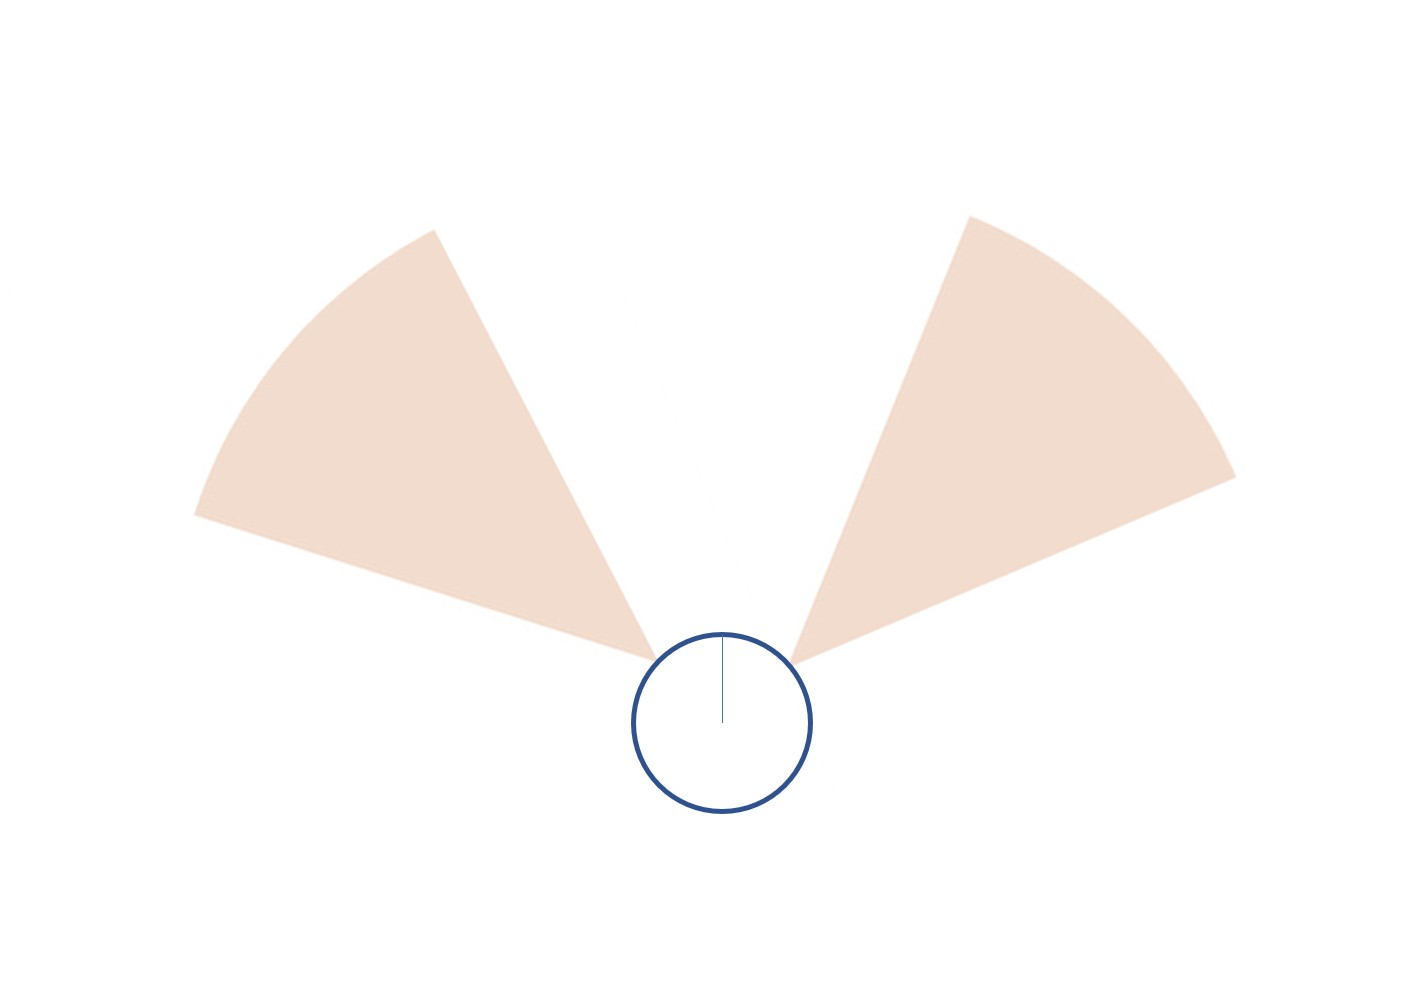
\includegraphics[scale=0.2]{img/robo.jpg}}}
      \caption{Schematic of the disk-shaped robot}
      \label{fig:robot}
   \end{figure}
   
   
\subsection{Behaviour Architecture}

The robot follows a simple subsumption based architecture.

   \begin{figure}[thpb]
      \centering
      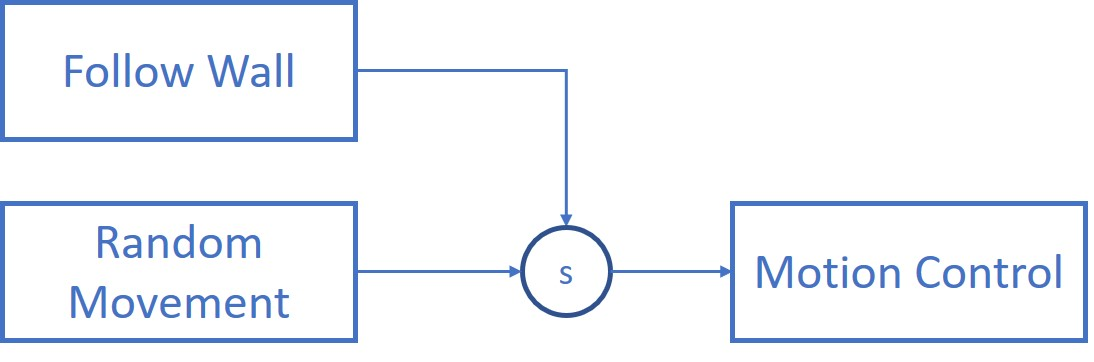
\includegraphics[scale=0.265]{img/architecture.jpg}
      \caption{Subsumption architecture}
      \label{fig:architecture}
   \end{figure}

The architecture has two different states, as shown in the figure \ref{fig:architecture}: \textit{random movement} and \textit{follow wall}. The robot will begin with an initial movement characterized by a random linear speed $\nu$ and a random angular speed $\omega$. It will maintain this random movement up until it first discovers a wall. When it detects an obstacle, the robot will follow along its walls indefinitely. The implemented algorithms that dictate the two states are described in the following section. 


\subsection{Algorithms}
\subsection{Initial random movement}\label{subsec:initial}

Until it finds the wall, the robot moves randomly, that is, at each step it chooses random linear and angular velocities. Depending on the initial distance of the robot to the nearest wall and its orientation, this random search may take a long time. 

We believe this wall finding time could be improved by making it more likely for the robot to move forward than for it to turn. This is clear if the robot is inside the wall it is suppose to find, like when it is inside the large D or between both D's. But in the case where the robot is outside the small D, going forward with higher probability might increase the likelihood of the robot finding the square walls delimiting the map, before it found the D walls.

Since the map delimiting wall is only there to stop the robot from trying to leave the map and not to be followed, we kept the robot moving randomly. In any case, the only downside is longer waiting time.

\subsection{Follow wall}
Upon discovering an obstacle the goal of the robot is to follow an imaginary line at a distance $D_i$ from the wall. 

   \begin{figure}[thpb]
      \centering
     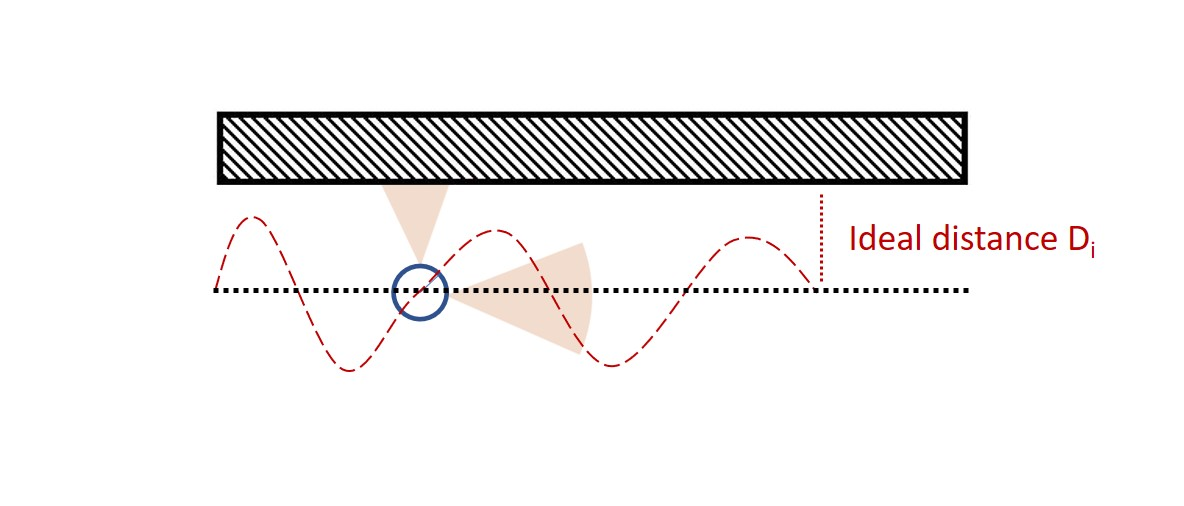
\includegraphics[scale=0.3]{img/behaviour.jpg}
      \caption{Robot behaviour following a wall}
      \label{fig:wall}
   \end{figure}

To do so, the robot uses the readings from the lasers to correct its trajectory. Knowing from which of the sensors is coming the measurements, the robot knows if the wall is on its right or left side and can act accordingly. If the robot is coming to close to the wall, the angular velocity takes the current symmetric value. The same happens if the robot begins to stray too far from the wall. In both cases, the linear velocity is maintained. This behavior reflects in a trajectory like the one in figure \ref{fig:wall}. When the robot loses the readings from the laser, we know we are present in a corner of the map. In order to keep following the wall, we have to perform what we call a ``hard turn''. In this case, the robot duplicates its standard angular velocity and reduces to 10\% of its normal linear speed.

\subsection{Maps}
Three maps were developed to test the robot. 
%%TODO: describe maps - what size? resolution = 0.05;

   \begin{figure}[thpb]
      \centering
     
\includegraphics[scale=0.2]{img/DD.png}
      \caption{The DD map}
      \label{fig:DD_map}
   \end{figure}
   
      \begin{figure}[thpb]
      \centering
     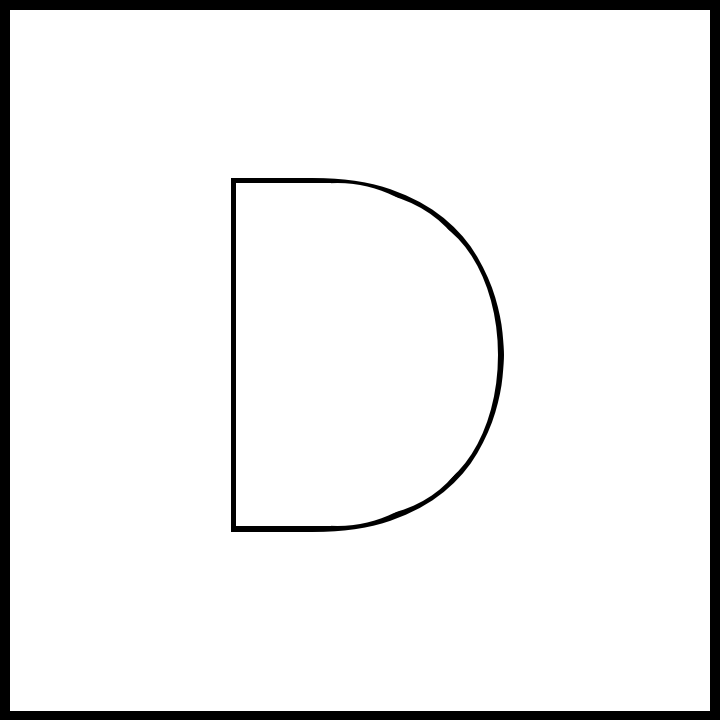
\includegraphics[scale=0.2]{img/inD.png}
      \caption{The inD map}
      \label{fig:inD_map}
   \end{figure}
   
   \begin{figure}[thpb]
      \centering
     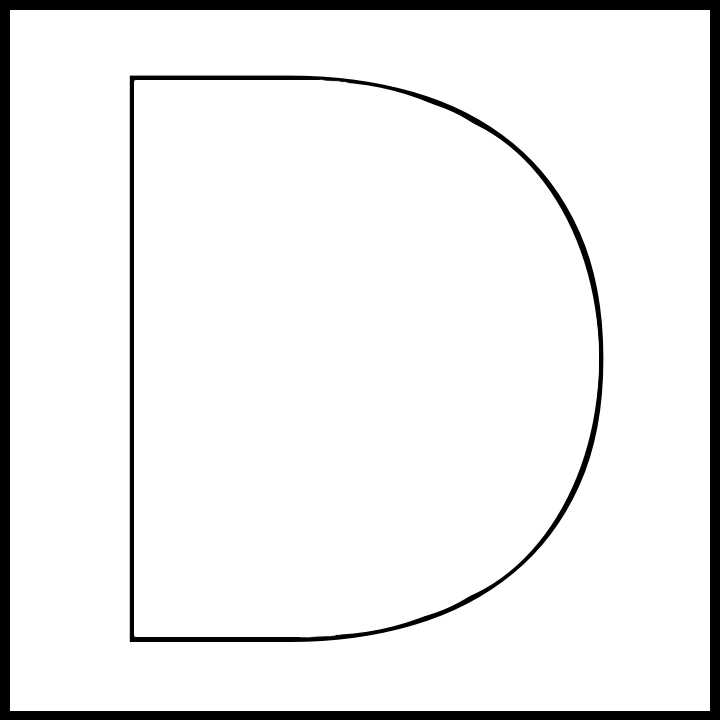
\includegraphics[scale=0.2]{img/outD.png}
      \caption{The outD map}
      \label{fig:outD_map}
   \end{figure}




%%%%%%%%%%%
% RESULTS %
%%%%%%%%%%%
\section{Results}
For each map, the robot will be place in a predefined position, before initiating its random movement. To validate the solution, we were interested in testing the ability of the robot to properly follow the wall present in each map and the stability of the algorithm. 
The ideal distances were set to $1m$ for the inD and outD maps and $2m$ for the DD map. For all cases, it was allowed and error of $0.1$ from the ideal distance. The distance to the wall was measured as the robot followed the wall, resulting in the following graphs.
 
   \begin{figure}[thpb]
      \centering
     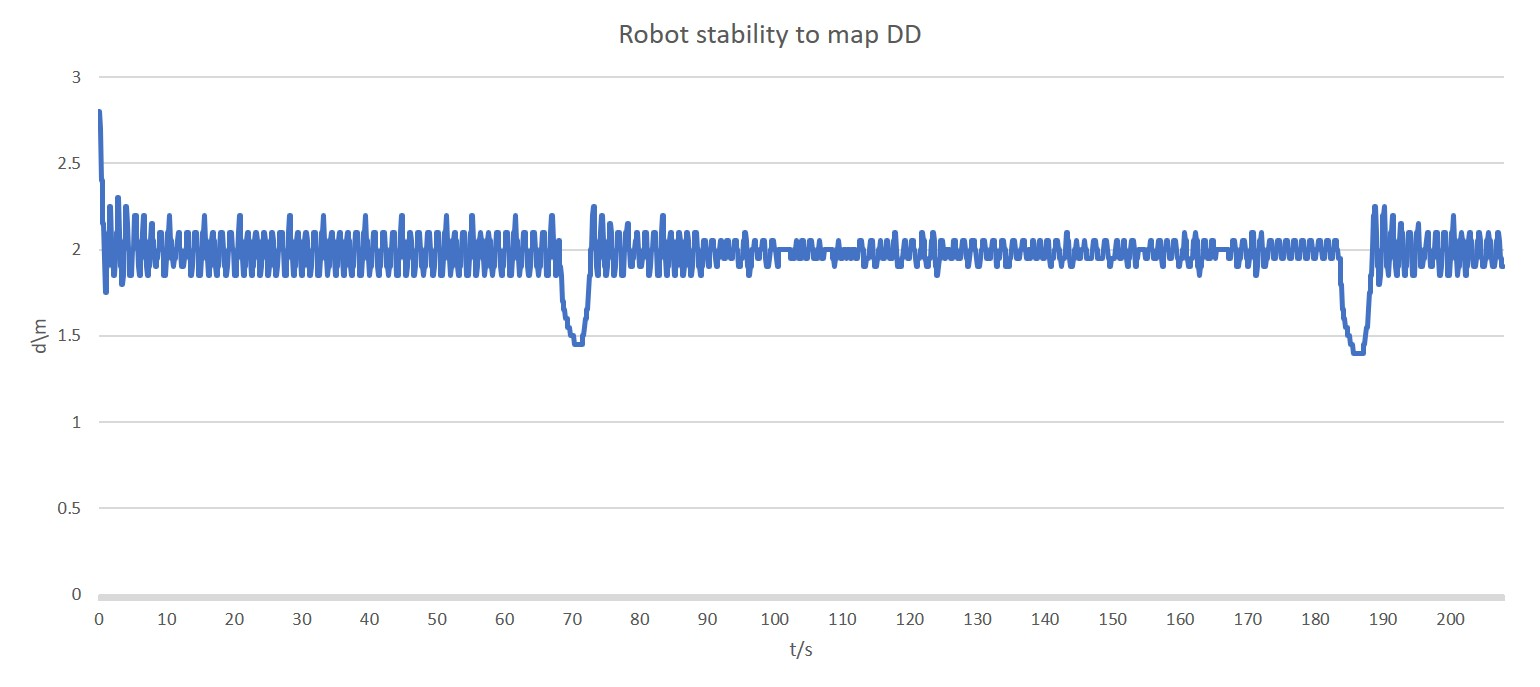
\includegraphics[scale=0.2]{img/map_DD.jpg}
      \caption{Robot stability to map DD}
      \label{fig:result_DD_map}
   \end{figure}
   
      \begin{figure}[thpb]
      \centering
     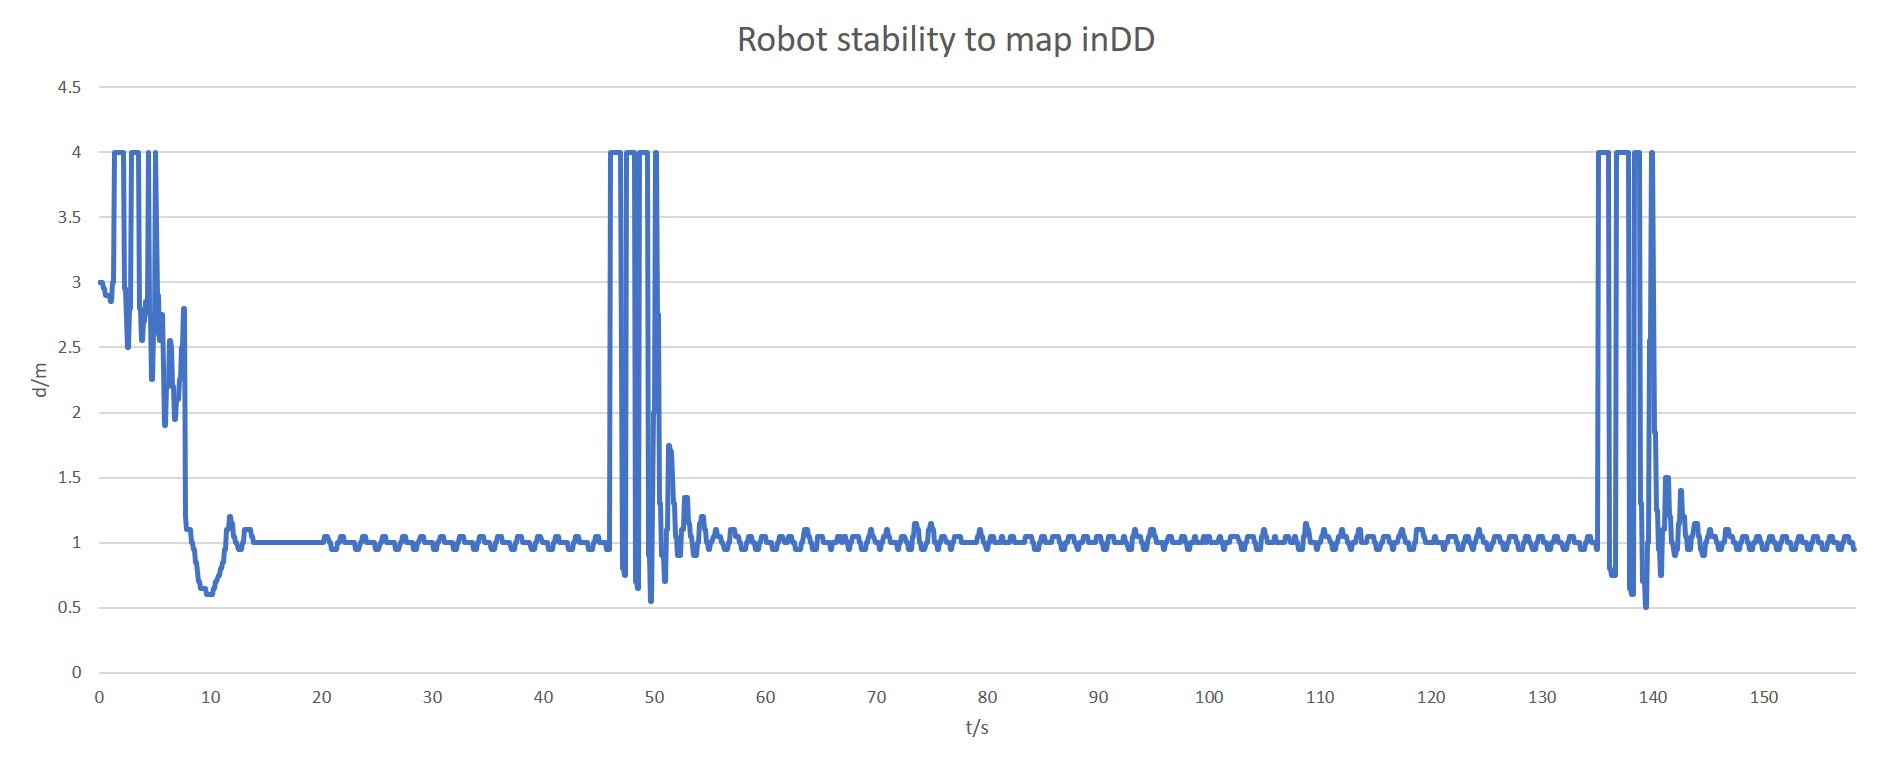
\includegraphics[scale=0.19]{img/map_inD.jpg}
      \caption{Robot stability to map inD}
      \label{fig:result_inD_map}
   \end{figure}
   
   \begin{figure}[thpb]
      \centering
     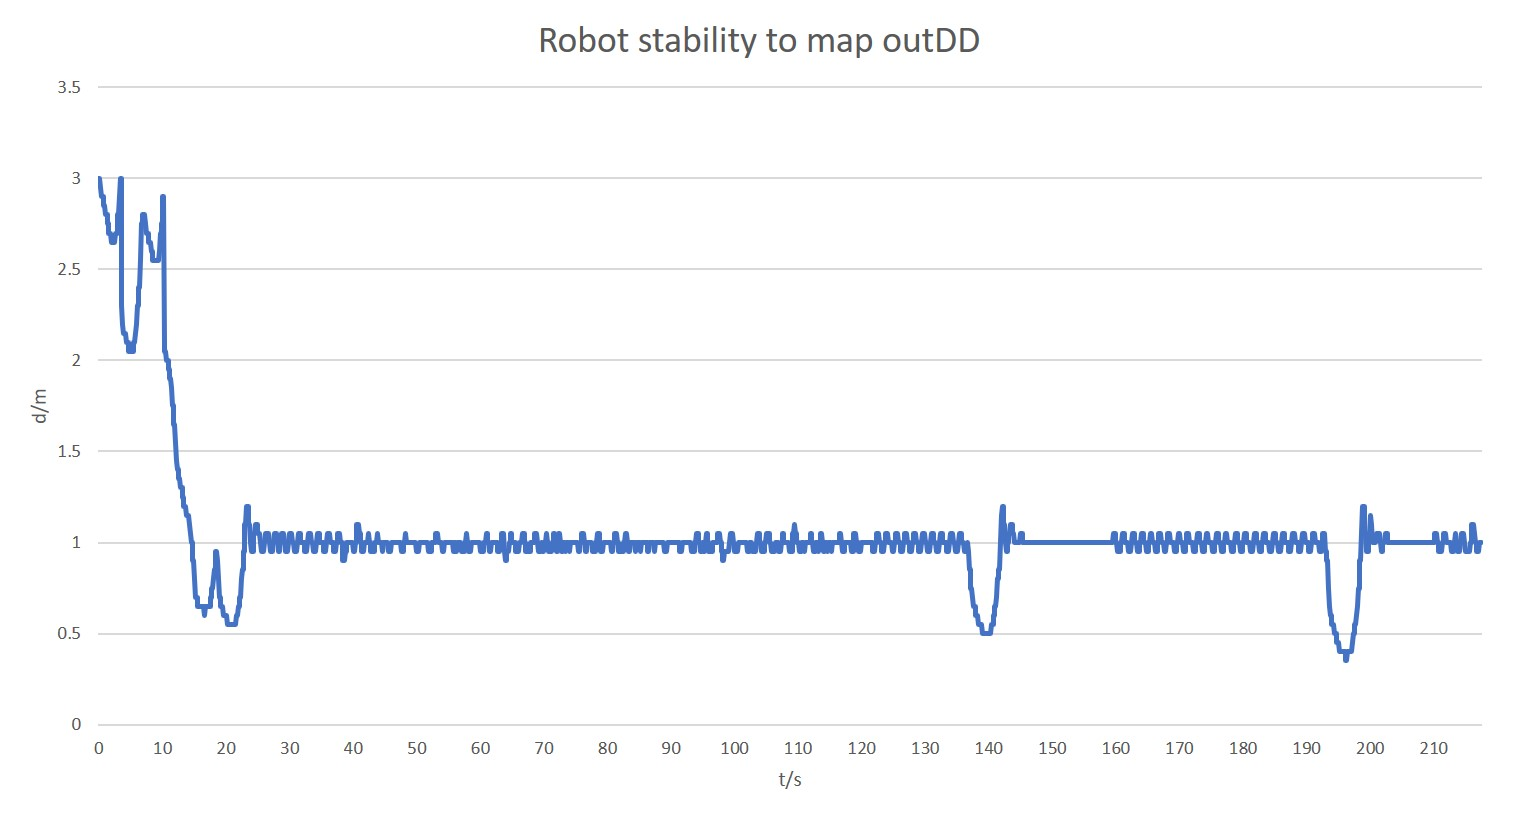
\includegraphics[scale=0.2]{img/map_outD.jpg}
      \caption{Robot stability to map outD}
      \label{fig:result_outD_map}
   \end{figure}



%%%%%%%%%%%%%%%
% LIMITATIONS %
%%%%%%%%%%%%%%%
\section{Limitations}

Nothing is perfect and our wall following robot is not an exception. Most of the limitations we detected in our robot are due to the simple ideas we used to make it work. However, we still believe that the simplicity of the code is worth the restrictions it creates.

\subsection{Map delimiting walls}

In order to keep the robot from trying to leave the map, we had to create squared walls around the map. These walls are not the ones the robot is supposed to find and follow, but if it does find these walls it will follow them forever.

Of course this only happens for the small D, whose walls the robot is supposed to follow from the outside. In the cases where the robot is inside the large D or between the two D's, it cannot move through those walls, therefore it will never find and follow the square map delimiting walls.

For the small D, we defined an initial position for the robot that is closer to the D than to the outside wall, although it sees neither of these walls. Thus, even though the initial movement of the robot will be random, it is more likely to find the small D wall and follow it. In case it finds the outside wall, the program should be stopped, but if it is not, the robot will still follow the outside wall without any problem.

\subsection{Desired wall distance}

The distance the robot tries to keep from the wall can be configured by the user. If the chosen distance is too small, the robot may not be able to turn on sharp corners. This happens because while turning the robot gets too close to the wall and perceives that it has run into it, which makes it stop altogether.

Perhaps there is some way to make the robot resume its movements if it runs into a wall, but we did not pursue that. Especially because the correct way to handle this would have been to force the robot to avoid all obstacles, which we also did not try.

As an example, for the large D that the robot follows from the inside, if the defined distance to the wall is 0.6 or less, the robot runs into the wall at the left corners of the D.

Although we did not test it, we are convinced that for smaller angled corners, the desired distance that the robot should keep from the wall must increase in order for it not to crash.

\subsection{Initial robot position}

If the initial position of the robot is on top or too close to a wall, it will not move. This is related to the previous limitation, as we did not try to get it to move after running into a wall. So the only way to avoid this error is to make sure that a safe initial position is configured for the robot, according to each map.

\subsection{Following two walls}

When the robot is between two walls, like when it is between the two D's, it does not follow both, that is it does not try to keep itself in the middle of both walls. We are not sure if that was the intention of the two D's assignment, but such behavior does make sense to us. The problem with trying to stay in the middle of two walls is that such behavior is different from that of trying to follow a wall at a given distance. 

There are two reasons why the robot may receive data from both lasers: either each laser detects a different wall, that is, the robot is between two walls; or both lasers detect the same wall, which may happen because the robot is facing the wall or because it is at a corner. Our way of dealing with data from both lasers is to use the laser that is closest to a wall. Unless the robot has already chosen a laser, in which case it should stick to it. This way, we avoid running into a wall because we where paying attention to the wrong laser. We also avoid turning around in an inner corner, because suddenly the other laser is closer to the wall. Plus, when the robot is facing a wall, it will eventually chose one laser, which means it will chose a direction in which to follow the wall. Unfortunately, it also means that when it is between two walls, the robot will pick the closest wall and follow it. To change this behavior, we need to be able to distinguish between the two scenarios above, and honestly we did not think further about this.

\subsection{Facing a wall}

When the robot first detects and approaches a wall, most often it will start to face that wall. Then as it goes towards the wall, because it is still further away from the wall then the desired distance, it does so in a peculiar way. Instead of going forward, it turns considerably left and right while approaching the wall.

We believe this behavior is explained by the way the robot chooses which laser to use. Suppose it chooses the left laser, then, since it is too far away from the wall, it quickly turns left, effectively making the left laser loose sight of the wall. Hence, it starts using the right laser, quickly turning right to get closer to the wall and possibly making the right laser loose sight of the wall. This may happen a few times, but eventually the robot is close enough that when turning, the chosen laser will not loose sight of the wall, leading to a normal behavior from then on.

We tried to fix this, making to robot stick to the first laser it chooses. But then it just started going around, because it had lost sight of the wall. So, although it is a strange way of going towards the wall, we kept it, because it works.

\subsection{Following a straight wall}

Sometimes, when the robot is following a straight wall, it will not go strictly forward, but very slightly deviate left and right. This is due to the noise from the lasers, and the error margin we use. We use a 0.01 error margin to quickly fix small deviations from the wall by turning $\pi/8$. If the noise is greater than 0.01, the robot will think it is too close or too far from the wall and turn a bit.

The reason for the error margin of 0.01 is because it makes the robot behave better when the wall does turn, that is, the robot follows the wall keeping a distance very close to the desired one. This happens even in sharp outer corners, that is when the robot needs to turn $\pi/2$.


%%%%%%%%%%%%%%%
% CONCLUSION %
%%%%%%%%%%%%%%%
\section{Conclusion}



\ifCLASSOPTIONcaptionsoff
  \newpage
\fi

%%%%%%%%%%%%%%%%
% BIBLIOGRAPHY %
%%%%%%%%%%%%%%%%
\bibliographystyle{IEEEtran}
\bibliography{IEEEabrv,wall_bib}

\end{document}